% !TEX root = paper.tex
% !TEX encoding = UTF-8 Unicode

\begin{figure*}
\begin{subfigure}[b]{.5\linewidth}
\begin{center}
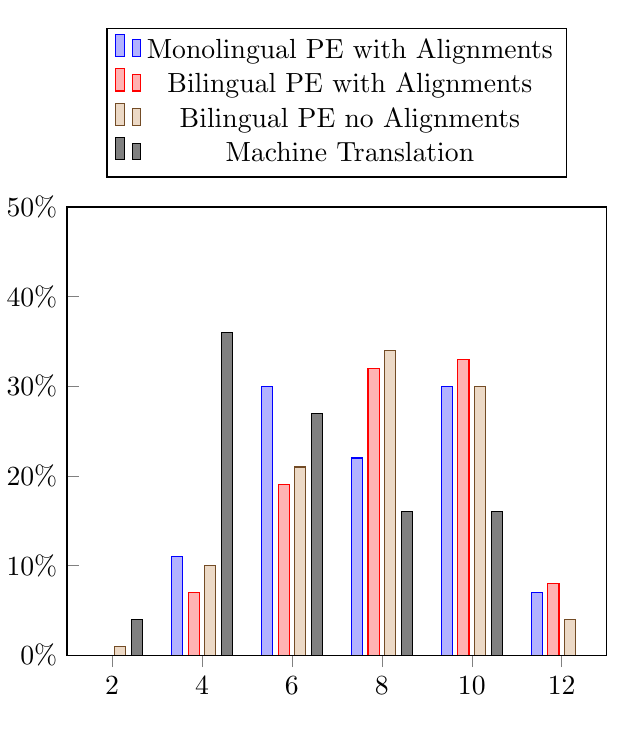
\begin{tikzpicture}[trim left={(-0.5,0)}]
\begin{axis}[
	%at={(10,0)},
	ymin=0,
	x tick label style={
		/pgf/number format/1000 sep=},
	ylabel shift={-0.15cm},
	ytick={0,10,20,30,40,50},
	yticklabels={0\%,10\%,20\%,30\%,40\%,50\%},
%	ymin={0},
	ymax={50},
%	ylabel={\%},
%	enlargelimits=0.15,
	xtick pos=left,
	ytick pos=left,
%	xlabel={XXXX YYY ZZZZ},
	%,
%	legend style={at={(0.5,-0.15)}},
%		anchor=north,legend columns=-1},
	legend style={at={(0.5,1.40)},anchor=north},
	ybar,
	bar width=4pt,
]
\addplot 
	coordinates {(4,11) (6,30) (8,22) (10,30) (12,7)};

\addplot 
	coordinates {(4,7) (6,19) (8,32) (10,33) (12,8)};

\addplot 
	coordinates {(2,1) (4,10) (6,21) (8,34) (10,30) (12,4)};

\addplot 
	coordinates {(2,4) (4,36) (6,27) (8,16) (10,16)};

\addplot[black,sharp plot,update limits=false] 
	coordinates {(-1,0) (14,0)};
	
\legend{Monolingual PE with Alignments,Bilingual PE with Alignments,Bilingual PE no Alignments, Machine Translation}
\end{axis}
\end{tikzpicture}
\end{center}
\caption{Russian-English}
\label{fig:percentage_segments_ru}
\end{subfigure}
\begin{subfigure}[b]{.5\linewidth}
\begin{center}
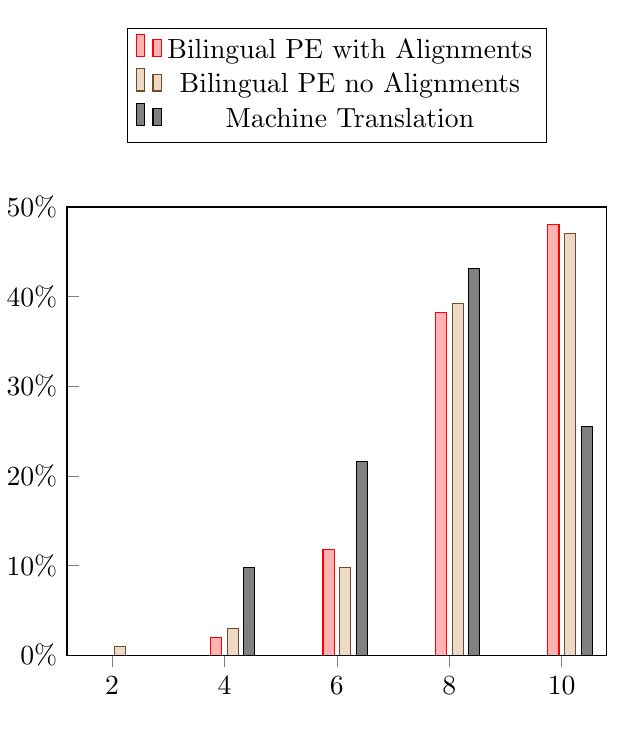
\begin{tikzpicture}[trim left={(-0.5,0)}]
\begin{axis}[
	%at={(10,0)},
	ymin=0,
	x tick label style={
		/pgf/number format/1000 sep=},
	ylabel shift={-0.15cm},
	ytick={0,10,20,30,40,50},
	yticklabels={0\%,10\%,20\%,30\%,40\%,50\%},
%	ymin={0},
	ymax={50},
%	ylabel={\%},
%	enlargelimits=0.15,
	xtick pos=left,
	ytick pos=left,
%	xlabel={XXXX YYY ZZZZ},
	%,
%	legend style={at={(0.5,-0.15)}},
%		anchor=north,legend columns=-1},
	legend style={at={(0.5,1.40)},anchor=north},
	ybar,
	bar width=4pt,
]
\addplot 
	coordinates {};

\addplot coordinates {(4,1.9607843137254901) (6,11.76470588235294) (8,38.23529411764706) (10,48.03921568627451) };
\addplot coordinates {(2,0.9803921568627451) (4,2.941176470588235) (6,9.803921568627452) (8,39.21568627450981) (10,47.05882352941176) };
\addplot coordinates {(4,9.803921568627452) (6,21.568627450980394) (8,43.13725490196079) (10,25.49019607843137) };

\addplot[black,sharp plot,update limits=false] 
	coordinates {(-1,0) (14,0)};
	
\legend{Bilingual PE with Alignments,Bilingual PE no Alignments, Machine Translation}
\end{axis}
\end{tikzpicture}
\end{center}
\caption{Spanish-English}
\label{fig:percentage_segments_es}
\end{subfigure}
\caption{\% of segments in each adequacy category.}
\label{fig:percentage_segments_en}
\end{figure*}
